\documentclass[11pt,a4paper]{article}
\usepackage{graphicx}
\usepackage[T1]{fontenc}
\usepackage[utf8]{inputenc}
\usepackage{lmodern,microtype}
\usepackage[a4paper,margin=21mm,top=20mm,bottom=22mm]{geometry}
\usepackage{amsmath,amssymb,booktabs,tabularx,array,enumitem,xcolor,titlesec,fancyhdr,hyperref}
\definecolor{ink}{HTML}{252923}
\definecolor{olive}{HTML}{526044}
\definecolor{muted}{HTML}{596253}
\color{ink}
\hypersetup{colorlinks=true,linkcolor=olive,urlcolor=olive,pdftitle={Fashion-MNIST: presentation script and defence guide},pdfauthor={Keoni}}
\urlstyle{same}
\def\UrlBreaks{\do\/\do\-\do\.\do\_}
\setlength{\emergencystretch}{2em}
\setlength{\parindent}{0pt}
\setlength{\parskip}{6pt}
\setlist[itemize]{leftmargin=*,nosep,topsep=4pt}
\setlist[enumerate]{leftmargin=*,itemsep=4pt,topsep=4pt}
\titleformat{\section}{\LARGE\bfseries\color{ink}}{}{0pt}{}
\titleformat{\subsection}{\large\bfseries\color{olive}}{}{0pt}{}
\titlespacing*{\section}{0pt}{0pt}{12pt}
\titlespacing*{\subsection}{0pt}{12pt}{4pt}
\pagestyle{fancy}
\fancyhf{}
\fancyhead[L]{\small Fashion-MNIST}
\fancyhead[R]{\small Rehearsal and defence}
\fancyfoot[R]{\thepage}
\renewcommand{\headrulewidth}{0.3pt}
\setlength{\headheight}{14pt}
\newcommand{\slide}[3]{\clearpage{\small\color{olive}SLIDE #1\hfill Target: #3}\par\section{#2}}
\newcommand{\say}{\subsection{Say aloud}}
\newcommand{\understand}{\subsection{Understand and defend}}
\newcommand{\screen}{\subsection{On screen}}
\newcommand{\selfcheck}[1]{\subsection{Check yourself}#1}
\newcommand{\transition}[1]{\par\smallskip\textit{Transition: #1}}
\newcounter{question}
\newcommand{\qa}[2]{\refstepcounter{question}\par\medskip\noindent\begin{minipage}{\linewidth}\textbf{\thequestion. #1}\par #2\end{minipage}\par}
\begin{document}
\thispagestyle{empty}
{\small\color{olive}A SPEAKING SCRIPT AND STUDY COMPANION}\par
\vspace{18mm}
{\Huge\bfseries Fashion-MNIST}\par\vspace{4mm}
{\LARGE How models see clothing}\par
\vspace{12mm}
{\Large Presentation script\\and defence guide}\par
\vspace{12mm}
Prepared for the feedback rehearsal with Professor \'Alvaro Rubio Garc\'ia. The spoken route follows the current sixteen-slide presentation, followed by four Q\&A slides; the explanations and question bank are supporting material.
\vspace{7mm}
\textbf{The story}\par
The same clothing images can be classified using nearby examples, weighted pixels or learned spatial patterns. A controlled comparison shows which approach performs best, while its errors show what the overall score hides.
\vspace{7mm}
\textbf{How to practise}
\begin{enumerate}
\item Read the ``Say aloud'' passage with the corresponding scene open.
\item Close the guide and explain the same idea in your own words.
\item Answer the check question before advancing. Use the final question bank to rehearse follow-ups.
\item Time one uninterrupted run. The planned route is \textbf{13 minutes}; this is a target, not a measured delivery time. Do not read the technical notes aloud.
\end{enumerate}
\vfill
\textbf{Evidence rule}\par
Results below come from saved project outputs. No retraining, new test-based selection or invented measurements are needed for this guide. Distinguish what was measured from what might explain it.

\clearpage\section{Your route through the story}
\begin{tabularx}{\linewidth}{rXrr}
\toprule
 & Scene & Time & Finish\\\midrule
1 & How models see clothing & 0:45 & 0:45\\
2 & Fashion-MNIST & 0:35 & 1:20\\
3 & From an image to 784 numbers & 0:55 & 2:15\\
4 & Keeping the comparison fair & 1:10 & 3:25\\
5 & kNN: the nearest examples & 0:55 & 4:20\\
6 & Logistic regression: weighted pixels & 0:55 & 5:15\\
7 & Inside the CNN & 1:10 & 6:25\\
8 & Which pixels matter? & 0:40 & 7:05\\
9 & Choosing the settings & 0:45 & 7:50\\
10 & When training stops helping & 0:35 & 8:25\\
11 & Final test performance & 0:35 & 9:00\\
12 & Accuracy varies by category & 0:35 & 9:35\\
13 & Shirt recall and directional errors & 0:50 & 10:25\\
14 & Which regions push the CNN toward Coat? & 1:00 & 11:25\\
15 & What the experiment cannot establish & 0:50 & 12:15\\
16 & The CNN performed best overall & 0:45 & 13:00\\\bottomrule
\end{tabularx}
\subsection{Keep the professor's priorities visible}
Explain your actual choices and results. Avoid giving three textbook lectures about the models. The relevant questions are: what information did each model receive, which settings were selected and why, how was leakage avoided, and what do the errors tell us?
\subsection{Before the mock presentation}
\begin{itemize}
\item Open the self-contained HTML in a browser and check fullscreen there.
\item Start with the default validation example, Coat \#22, so the walkthroughs tell one connected story.
\item Know how to change examples, select CNN channels, change interpretation targets, watch the automatic occlusion scan, switch tuning tabs and show the confusion matrix. These are optional demonstrations, not invitations to explore indefinitely.
\item On the learning-curve scene, point to epoch 12, the retained checkpoint.
\item Keep the question bank available separately. Do not project it during the timed story.
\end{itemize}
\subsection{If you run long}
Keep the split, model choices, final results and shirt analysis. Keep the interpretation slide to its 40-second comparison. Shorten optional interactions, exact parameter arithmetic and seed details. Reserve detailed answers for discussion.

\slide{1}{How models see clothing}{45 seconds}
\say
We want to predict a clothing category from a picture. A catalogue could use that prediction to help organise new items. This is supervised multiclass classification: our target is one of ten clothing labels. Logistic regression is our baseline. We compare it with a nearest-neighbour classifier and a CNN to see what the extra complexity buys us and which mistakes remain.
\understand
\begin{itemize}
\item \textbf{Input $X$:} a grayscale clothing image. \textbf{Target $y$:} one of ten known categories.
\item \textbf{Learning setting:} supervised, because training images have labels; multiclass classification, because the output is a category rather than a continuous quantity.
\item \textbf{Motivation:} an image benchmark makes the difference between flat pixel features and spatial processing visible and measurable.
\item The comparison is useful, but it does not isolate convolution as the sole cause of improvement: model capacity and training also differ.
\end{itemize}
\screen
Let the image collage establish the subject. Name the three approaches; save their mechanics for their own scenes. Do not reveal every result in the opening.
\selfcheck{What is the model given, what must it predict, and why is this supervised classification?}
\transition{``First, what exactly are the images?''}

\slide{2}{Fashion-MNIST}{35 seconds}
\say
Fashion-MNIST gives us 70,000 labelled grayscale images in a common format. Its balance makes accuracy easy to interpret: each category has equal representation and we give each mistake equal cost. Accuracy is our primary metric. We also report macro-F1 and class recall because a good overall score can hide a weak category.
\understand
\begin{itemize}
\item Ten classes: T-shirt/top, trouser, pullover, dress, coat, sandal, shirt, sneaker, bag and ankle boot.
\item The development pool has 6,000 examples per class; the official test set has 1,000 per class.
\item A label is the dataset's reference category. The project measures agreement with those labels; it does not establish that every label is beyond debate.
\item Balanced categories prevent a majority category from dominating accuracy. They do not guarantee equal difficulty or fairness across people.
\end{itemize}
\screen
Point to a few real dataset images and the 70,000 / 10-category statistics. Avoid reciting all ten labels aloud.
\selfcheck{Why is this dataset useful for comparison, and why does success here not establish performance on phone photos?}
\transition{``Those small images still need to become model inputs.''}

\slide{3}{From an image to 784 numbers}{55 seconds}
\say
Each image has 784 unsigned eight-bit pixel values. The target is an integer category label. Our exploration found no missing values, invalid labels or exact duplicates in the development data. About half the training pixels are zero. We kept the observations and divided intensities by 255. That fixed transformation needs no fitted statistics. Logistic regression and kNN receive flattened pixels; the CNN receives the original grid in one channel.
\understand
\begin{itemize}
\item $28\times28=784$. Normalisation is $x'=x/255$, not standardisation by a fitted mean and standard deviation.
\item The scale factor is a known intensity bound; no validation or test statistic is fitted to compute it.
\item Flattening preserves the pixel values and their consistent ordering. It removes the \emph{explicit two-dimensional arrangement} from the input interface; logistic regression can still learn a weight for each fixed position.
\item Classical inputs are floating-point flat arrays; CNN inputs are float32 tensors with shape $(N,1,28,28)$.
\item Uniform scaling alone does not change Euclidean neighbour rankings. It standardises the numerical representation and supports optimisation for the trained models.
\end{itemize}
\screen
The pixel scan starts automatically, updating intensity, normalisation and its position in the flat vector. Point to the moving highlight; no hovering is needed. Explain the representation rather than narrating every pixel.
\selfcheck{Does flattening delete pixels? What spatial structure does a CNN explicitly exploit?}
\transition{``Before training, the data must be divided fairly.''}

\slide{4}{Keeping the comparison fair}{70 seconds}
\say
The publisher supplied the 10,000-image test set. We split the remaining 60,000 into 48,000 training and 12,000 validation images. We took the first split from StratifiedGroupKFold. Stratification preserved class proportions, and grouping would have kept identical images together. Each category was exactly ten percent of every split, so resampling was unnecessary. We used one validation holdout for tuning. We fitted the models on training data, compared candidate settings on validation, and froze the checkpoints before scoring the test set once.
\understand
\begin{itemize}
\item \textbf{Training} fits weights or stores kNN examples. \textbf{Validation} selects settings and checkpoints. \textbf{Test} evaluates the frozen choices.
\item Actual code: \texttt{n\_splits=5}, \texttt{shuffle=True} and \texttt{random\_state=42}. A single \texttt{next(...)} takes the first result from \texttt{splitter.split(...)}.
\item Groups use SHA-256 hashes of original uint8 image pixels. No duplicate groups were found; no duplicate-removal claim is warranted.
\item Source indices and split fingerprints make the comparison reproducible. Exact balance was verified here; arbitrary grouped data need not yield perfectly equal proportions.
\end{itemize}
\screen
Let the subset breakdown finish. Point to the equal 10\% shares. Keep ``one fixed split'' distinct from the five-fold implementation detail.
\selfcheck{What is the difference between stratification, grouping and cross-validation?}
\transition{``With the split fixed, the first model compares an image with stored examples.''}

\slide{5}{kNN: the nearest examples}{55 seconds}
\say
For kNN we tried three, five and nine neighbours. Three won on validation. Here two of the three nearest images are pullovers, so the coat is misclassified. To measure training accuracy, each image voted using only the three nearest other images. That gave 85.27 percent, close to 85.04 percent on test. Its test advantage over the logistic baseline was just 0.71 percentage points.
\understand
\[
 d(x,z)=\sqrt{\sum_{j=1}^{784}(x_j-z_j)^2}.
\]
\begin{itemize}
\item Selected configuration: $k=3$, Euclidean distance, uniform weights, brute-force search.
\item Default example: validation Coat \#22. Neighbours: training \#31811 Pullover, \#37819 Pullover and \#2785 Coat. Distances approximately 4.836, 5.038 and 5.103.
\item Two of three votes is not a calibrated 66.7\% chance of correctness; it is the local vote fraction.
\item $k=3$ beat $k=5$ by only seven validation images. Describe a small observed advantage, not a universal optimum.
\item Ordinary training-set scoring includes the query itself as a neighbour. Excluding each query by index gives 40,931 correct out of 48,000 (85.27\%).
\end{itemize}
\screen
Use the same coat throughout the three walkthroughs. Point to the labels of its neighbours and the resulting vote; replay once if useful.
\selfcheck{Why can kNN misclassify this coat even though the nearest images look similar?}
\transition{``The next model learns how much each pixel position should contribute.''}

\slide{6}{Logistic regression: weighted pixels}{55 seconds}
\say
Logistic regression gives each pixel a weight for each class. Adding the weighted pixels and intercept gives a class score. The heatmap shows contributions to the predicted score. Of four L2 regularisation settings, C equal to 0.1 had the highest validation accuracy. Our baseline reached 87.42 percent on training and 84.33 percent on test. Its three-point gap is modest. A linear score also limits how this model can combine neighbouring pixels into patterns.
\understand
For class $c$, the model forms a logit $z_c=w_c^Tx+b_c$, then uses multiclass softmax:
\[
 p_c=\frac{e^{z_c}}{\sum_{r=1}^{10}e^{z_r}}.
\]
\begin{itemize}
\item L2 penalises large weights. Smaller $C$ means stronger regularisation in this implementation; $C$ is not a learning rate.
\item Tried $C\in\{0.01,0.1,1,10\}$; selected validation accuracy 85.40\%. The gain over $C=1$ was just ten images.
\item The solver is LBFGS, with maximum 2,000 iterations. The selected run converged; an iteration is not a CNN epoch.
\item A contribution is $w_{cj}x_j$, not the weight alone and not a causal explanation. Softmax probabilities are not proven calibrated confidence estimates.
\end{itemize}
\screen
Show the input, contribution map and probability ranking. If asked, the displayed class score is the sum of contributions plus its bias.
\selfcheck{What does changing $C$ do, and why does this remain a classification model despite its name?}
\transition{``The CNN instead learns local patterns while preserving the image grid.''}

\slide{7}{Inside the CNN}{70 seconds}
\say
The CNN keeps the grid. The first convolution learns 32 local filters and the second learns 64. Pooling reduces the spatial dimensions, then a 128-unit dense layer combines the features. We used dropout of 0.25 and restored epoch 12. At that checkpoint accuracy was 95.67 percent on training and 91.79 percent on test. That is a 7.46-point gain over our baseline. The remaining train-to-test gap motivated a closer look at the learning curves.
\understand
\[
1\!\times\!28\!\times\!28\ \longrightarrow\ 32\!\times\!14\!\times\!14\
\longrightarrow\ 64\!\times\!7\!\times\!7\ \longrightarrow\ 3136\ \longrightarrow\ 128\ \longrightarrow\ 10.
\]
\begin{itemize}
\item Two convolutional \emph{layers}, not 96 separate networks. Channels are learned feature responses.
\item Padding one preserves width and height during each convolution. Pooling halves them.
\item ReLU is $\max(0,x)$. Leaky ReLU was not evaluated; do not claim ReLU won an activation comparison.
\item The last layer outputs raw logits. PyTorch cross-entropy handles the required log-softmax internally; displayed probabilities are computed with softmax afterwards.
\item The filter scan is illustrative. Maps are saved forward-pass outputs, not live retraining. Intensities share a scale within each recorded layer tensor, not across layers.
\end{itemize}
\screen
Follow input, first block, second block and class output. Show one channel change at most. Do not assign an unverified semantic meaning to each map.
\selfcheck{Why are ReLU and softmax used in different places, and how many convolutional layers are there?}
\transition{``We can also ask which input pixels affect a chosen class score.''}

\slide{8}{Which pixels matter?}{40 seconds}
\say
For this coat, gradient saliency highlights pixels where a small change would most affect the Coat score. Occlusion asks what happens to the same score when we cover a patch. As the patch moves, the readout shows the change in the raw score. Both maps describe sensitivity for this image. Later we will use SHAP to measure signed contributions to a probability.
\understand
\begin{itemize}
\item \textbf{Gradient:} $S_{ij}=\left|\partial z_c/\partial x_{ij}\right|$, the magnitude of sensitivity of raw class logit $z_c$ to normalised input pixels. It is not a probability or a segmentation mask.
\item \textbf{Occlusion:} $\Delta z_c=z_c(x)-z_c(x_{\mathrm{covered}})$. Positive means covering the patch reduced the fixed target score; negative means it increased. The pixel map averages signed drops across covering patches, then displays positive values only. The patch readout retains the sign.
\item Patches are $5\times5$, stride 2, fill 0.5 on $[0,1]$; the final edge position is included. These are diagnostic choices, not validated optimal settings. Gray patches may create unnatural inputs.
\item Each map is normalised independently for display: equally bright regions across different images or methods do not imply equal numerical sensitivity. Absolute gradients also omit direction.
\item Validation Coat \#22 is the default; Shirt \#32 was already among the ten fixed examples. Do not select new examples because their maps look convincing.
\end{itemize}
\screen
Keep Coat selected, compare the maps and let the patch scan play automatically. It starts on entry and pauses when leaving or opening notes. If time permits, select Shirt and switch the target from predicted Coat to actual Shirt. Reserve extended exploration for questions.
\selfcheck{What does a positive occlusion score drop mean, and why must the target class stay fixed?}
\transition{``Interpretation explains a fixed model; validation evidence explains why we chose its settings.''}

\slide{9}{Choosing the settings}{45 seconds}
\say
We chose settings on validation accuracy. Within each CNN run we restored the epoch with lowest validation loss. Across configurations, the wider CNN without weight decay won. The two wider versions were very close across three seeds, and weight decay had higher mean shirt recall. We retained the original accuracy-first choice. Those seeds measure training variation on the same split.
\understand
\begin{tabularx}{\linewidth}{Xr}
\toprule CNN configuration & Validation accuracy\\\midrule
Original baseline & 90.70\%\\
Original extended & 91.45\%\\
Wider, retained & 92.33\%\\
Wider with weight decay & 92.28\%\\\bottomrule
\end{tabularx}
\begin{itemize}
\item Two architecture widths, four initial training runs, then four additional seed runs: eight runs total. Each wider configuration has seeds 42, 7 and 123, reusing its original seed-42 run.
\item Mean validation accuracy: wider 92.400\%, weight decay 92.339\%. Sample standard deviations: 0.347 and 0.059 percentage points. Three seeds measure limited training randomness, not split uncertainty or a confidence interval.
\item These were practical bounded choices, not exhaustive searches. Test results were not the basis for selecting these settings.
\end{itemize}
\screen
Briefly switch the comparison tabs. Do not read every table cell or every seed statistic.
\selfcheck{Why can the best validation-loss checkpoint differ from the epoch with the best accuracy?}
\transition{``The learning curves explain why the final epoch was not automatically the best.''}

\slide{10}{When training stops helping}{35 seconds}
\say
Training loss continued falling after epoch 12. Validation loss reached its minimum there, so later epochs improved training fit without improving that criterion. Training stopped at epoch 17 and restored epoch 12. That divergence is evidence of overfitting with further training.
\understand
\begin{itemize}
\item One epoch means one pass through the training subset. A batch is a smaller group used for an optimisation update; batch size is 128.
\item Adam starts with learning rate 0.001. ReduceLROnPlateau halves it after two plateau epochs under its configured rule; early stopping uses patience five. These are different mechanisms.
\item Loss reflects probabilities and penalises confidently wrong predictions. Accuracy depends only on the winning class. Epoch 16 could have higher accuracy without lower loss.
\item LR: training 87.42\%, validation 85.40\%; this modest gap alone does not prove severe overfitting or pure underfitting. Limited linear capacity is a plausible restriction.
\item kNN: do not infer a clean fit diagnosis from self-inclusive training accuracy. Its validation result and pixel-distance limitation are directly defensible.
\end{itemize}
\screen
Point to the validation-loss minimum and move the epoch control only enough to show the later divergence. Return to epoch 12.
\selfcheck{Why restore epoch 12 instead of using the weights from epoch 17?}
\transition{``Once the models were fixed, we evaluated the official test set.''}

\slide{11}{Final test performance}{35 seconds}
\say
The summary shows the size of the improvement. kNN gains less than one point over logistic regression. The CNN gains more than seven and also leads on macro-F1. It had already won on validation; final testing confirmed the choice. Which items does it still miss?
\understand
\begin{tabularx}{\linewidth}{Xrrr}
\toprule Model & Validation & Test & Test macro F1\\\midrule
Logistic regression & 85.40\% & 84.33\% & 0.8424\\
kNN & 85.38\% & 85.04\% & 0.8502\\
CNN & 92.33\% & 91.79\% & 0.9167\\\bottomrule
\end{tabularx}
\begin{itemize}
\item CNN: 9,179 correct and 821 incorrect. Accuracy is total correct divided by total images.
\item $91.79-85.04=6.75$ \emph{percentage points}, not 6.75\% relative improvement.
\item Frozen evaluation used retained models trained on 48,000 images; there was no refit on all 60,000 development images.
\item A prior test-file integrity check was not model scoring. Final evaluation checked saved-model provenance and validation parity before test scoring.
\item Once test performance is known, changing settings to improve that score would contaminate its role as an independent final assessment.
\end{itemize}
\screen
Pause on the results. Compare gains over the baseline and explain why the ranking matters. Keep validation and test values distinct.
\selfcheck{What can the test result establish, and why should it not be used for another tuning round?}
\transition{``But one overall score can hide a difficult category.''}

\slide{12}{Accuracy varies by category}{35 seconds}
\say
Each confusion-matrix row starts with a thousand actual items. Read across a row to see the predictions. The CNN recognises 99 percent of bags but only 67.6 percent of shirts. Equal class sizes make that difference particularly easy to interpret.
\understand
\[
\operatorname{recall}_c=\frac{TP_c}{TP_c+FN_c},\qquad
\operatorname{precision}_c=\frac{TP_c}{TP_c+FP_c}.
\]
\begin{itemize}
\item Recall starts with \emph{actual members}; precision starts with \emph{predicted members}. Do not swap the denominators.
\item A row-normalised confusion matrix divides each row by its actual-class total. Here that denominator is 1,000 for every class.
\item With equal class sizes, macro recall equals overall accuracy mathematically. Macro F1 can differ because it also incorporates precision and the nonlinear F1 formula.
\item Do not say the CNN wins every class: kNN ankle-boot recall is 97.3\%, versus 97.0\% for the CNN, a three-image difference.
\end{itemize}
\screen
Select Shirt, briefly compare with Bag, then show the matrix and identify one diagonal and one off-diagonal cell. Return to Shirt if needed.
\selfcheck{What is the difference between ``67.6\% of actual shirts were found'' and ``67.6\% of predicted shirts were correct''?}
\transition{``The shirt errors have a clear directional pattern.''}

\slide{13}{Shirt recall and directional errors}{50 seconds}
\say
Of the thousand actual shirts, 324 were missed. Look at the first pair: 127 shirts were called T-shirt or top, while only 63 T-shirts or tops were called shirt. The same asymmetry appears for coats and pullovers. Similar outlines are a plausible explanation at this low resolution. The counts establish the direction of the errors; the images alone cannot establish their cause.
\understand
\begin{tabularx}{\linewidth}{Xrr}
\toprule Other category & Shirt $\to$ other & Other $\to$ Shirt\\\midrule
T-shirt/top & 127 & 63\\
Coat & 89 & 32\\
Pullover & 71 & 32\\\bottomrule
\end{tabularx}
\begin{itemize}
\item $127+89+71=287$ of the 324 missed shirts; 37 went to other categories. These pairs do not exhaust all mistakes.
\item Bars share a zero origin and scale. Each arrow reads \emph{actual $\to$ predicted}; both source classes have 1,000 images.
\item Directional examples are the first saved test index matching each error, not a random or representative sample: outgoing shirt IDs 474, 117, 244; reverse IDs 381, 324, 49 respectively.
\item Pictures cannot prove causation, greater within-class variation or incorrect ground-truth labels.
\end{itemize}
\screen
Point to one image pair and read its two directions. State the remaining pairs briefly. Keep ``observed'' separate from ``plausible explanation''.
\selfcheck{How can the classes be balanced while shirt errors are both more frequent and asymmetric?}
\transition{``What pushed the CNN toward Coat on one validation shirt?''}

\slide{14}{Which regions push the CNN toward Coat?}{60 seconds}
\say
Both SHAP plots explain the CNN's Coat probability. On the left, each dot is one validation image. Its horizontal position shows how much that quadrant raised or lowered the probability. Colour gives its average brightness. Across these 100 images, upper right has the largest average absolute effect. On the right is one actual shirt predicted as Coat. Starting at the training-reference average of 14.0 percent, all four quadrants push toward Coat, reaching 58.3 percent. For this shirt, lower right contributes most, about 15.5 percentage points. The answer depends on our region boundaries and reference images.
\understand
The four features are $14\times14$ quadrants. For each of the 16 subsets, keep those regions from the image and fill the rest from one training reference at a time. Average Coat probability over 20 references, two per class. The Shapley value averages the change from adding a region over all possible orders. Values are exact for this four-region game and its finite background.
\begin{center}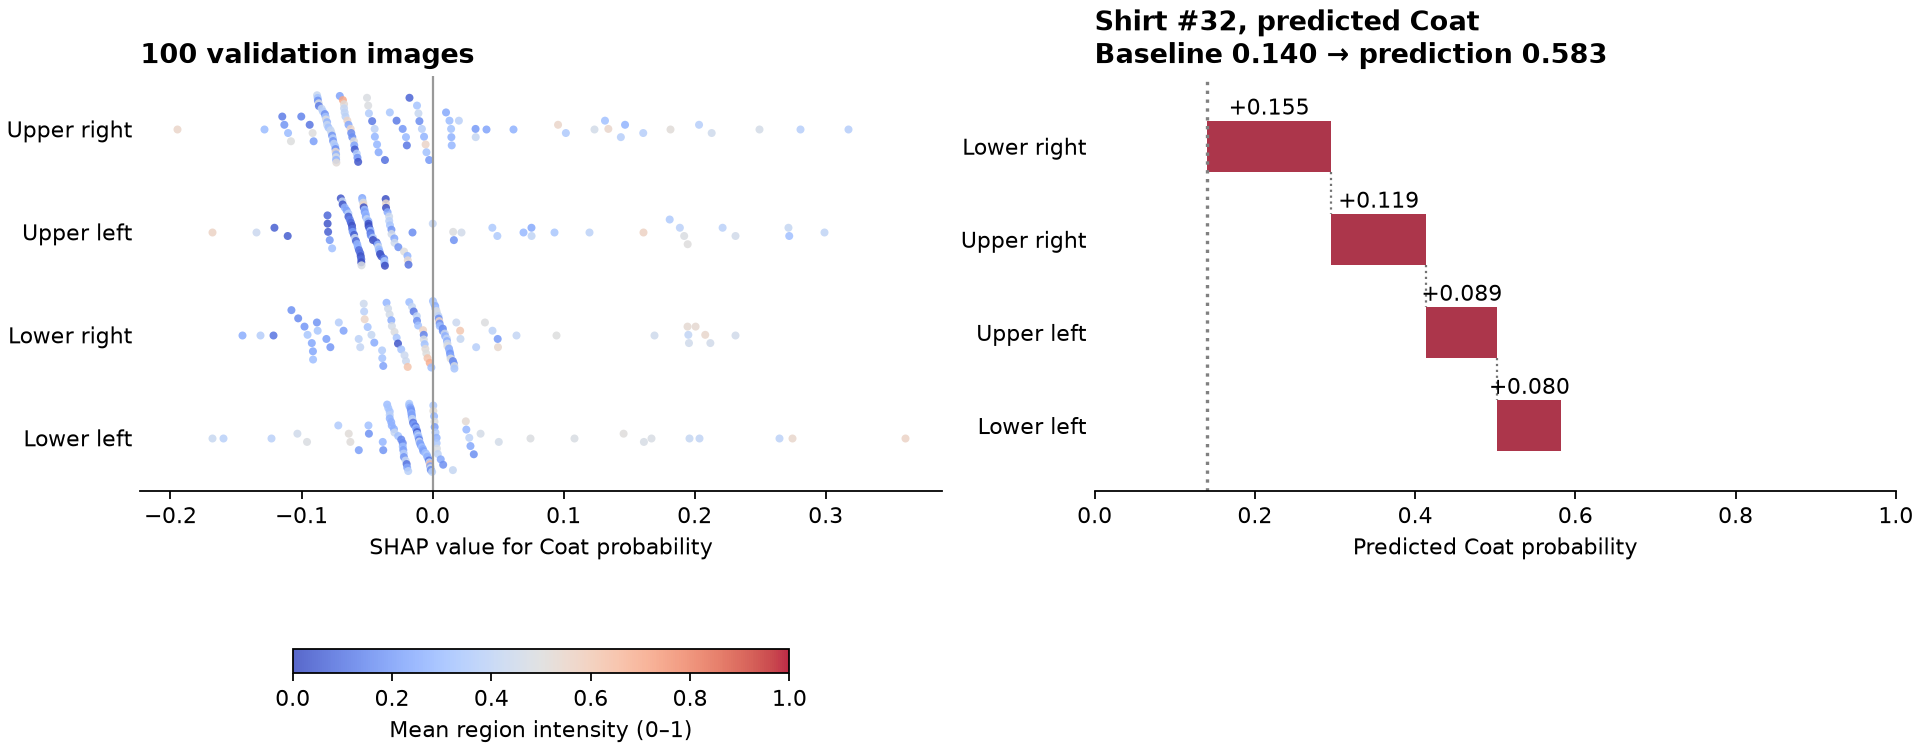
\includegraphics[width=\linewidth]{../editorial/coat-shap.png}\end{center}
\screen
Read the beeswarm horizontally. Each row is a region; colour is its mean intensity. Read the waterfall from its baseline through four contributions. Mixed-quadrant images can be unrealistic. The background and region boundaries affect the result. See W12, pages 28--29.
\selfcheck{Why can upper right rank first across images while lower right contributes most to this shirt?}
\transition{What are the limits of these findings?}

\slide{15}{What the experiment cannot establish}{50 seconds}
\say
We used one validation split, so repeated choices could adapt to those images. The CNN also differs from the other models in capacity and training, so the comparison cannot isolate the benefit of convolution alone. Fashion-MNIST contains small, standardised images. My next experiment would evaluate the frozen CNN on independently labelled phone photos with different lighting and backgrounds.
\understand
\begin{itemize}
\item A seed changes aspects of training randomness. A new split changes which images support fitting and validation. They assess different sources of variability.
\item No exact overlap is a narrower statement than ``no leakage of any kind'' or ``no near duplicates''.
\item Improvement ideas are future experiments: additional validation splits, controlled ablations or genuinely new image data. The present test should not become a tuning target.
\item Balanced labels say nothing about demographic coverage, whose attributes were not measured here.
\end{itemize}
\screen
Use the four visible limitations as the structure. Avoid adding a long list of speculative future projects.
\selfcheck{Why do three seeds not replace multiple validation splits?}
\transition{``Within those limits, the main conclusion is clear.''}

\slide{16}{The CNN performed best overall}{45 seconds}
\say
The CNN was the best of our three models on this benchmark. It improved test accuracy by 7.46 points over logistic regression. But if a catalogue particularly needs reliable shirt labels, overall accuracy hides a practical weakness: the CNN misses about a third of actual shirts. That is the result I would investigate before relying on it for new photographs. Thank you. What questions do you have?
\understand
\begin{itemize}
\item Strongest claim: best \emph{among the evaluated configurations on this benchmark}.
\item Keep the two memorable numbers attached to their metrics: 91.79\% overall test accuracy; 67.6\% test shirt recall.
\item The model comparison is empirical support, not proof that CNNs always win or that every improvement comes from convolution.
\end{itemize}
\screen
Pause, finish the sentence and stop. Use O to jump directly to Q\&A slides 17--20.
\selfcheck{Can you give the conclusion in two sentences without overstating what the experiment proves?}

\clearpage\section{Q\&A slide guide}
Stop after slide 16. Press \textbf{O} to open the index and choose the slide that matches the question. Budget one to two minutes for questions. These slides are outside the 13-minute route.

\subsection{17. How did you prevent leakage?}
Fit the classifiers. Divide raw pixel intensities by the known maximum of 255; this uses no estimated statistics. Choose C, k, CNN settings and checkpoint. All models use identical source indices. Only the first split from StratifiedGroupKFold was used. Freeze all three checkpoints, verify their hashes and validation predictions, then score once. Exact development/test overlaps: zero.
\subsection{18. How was kNN training accuracy measured?}
For each of the 48,000 fitted images, exclude its own index and search the other 47,999 images. Three Euclidean neighbours, one vote each. A three-way tie goes to the lowest class ID, matching the classifier. 40,931 $\div$ 48,000 = 85.27\%. Validation: 85.38\%. Test: 85.04\%. These close scores give little evidence of a large generalisation gap.
\subsection{19. Why keep the epoch-12 CNN?}
Validation loss reached its minimum at epoch 12. Training stopped at epoch 17 and restored that checkpoint. Validation accuracy chose the wider CNN without weight decay. The original seed-42 checkpoint was already selected. Mean accuracy: 92.400\% without weight decay and 92.339\% with it. Mean shirt recall favoured weight decay: 78.94\% vs. 75.81\%. All runs used one split.
\subsection{20. What do these SHAP values measure?}
The frozen CNN's Coat probability. One feature is a 14 $\times$ 14 quadrant. Absent quadrants come from the same reference image. Evaluate all 16 subsets of the four quadrants, averaging each over 20 training images (two per class). Average each region's marginal change over possible orders. The baseline plus four signed contributions recovers each prediction. The beeswarm covers ten validation images per class. Other backgrounds or region boundaries can change the values; mixed images may look artificial.

\clearpage\section{Technical reference}
This page is for follow-up questions, not the timed speech.
\subsection{Selected CNN, precisely}
\begin{tabularx}{\linewidth}{Xrr}
\toprule Layer & Output per image & Parameters\\\midrule
Conv2d: 1 to 32, kernel 3, padding 1 & $32\times28\times28$ & 320\\
ReLU, MaxPool2d(2) & $32\times14\times14$ & 0\\
Conv2d: 32 to 64, kernel 3, padding 1 & $64\times14\times14$ & 18,496\\
ReLU, MaxPool2d(2) & $64\times7\times7$ & 0\\
Flatten & 3,136 & 0\\
Linear: 3,136 to 128 & 128 & 401,536\\
ReLU, Dropout(0.25) & 128 & 0\\
Linear: 128 to 10 & 10 logits & 1,290\\\midrule
Total & & \textbf{421,642}\\\bottomrule
\end{tabularx}
For a convolution: $(k_hk_wC_{in}+1)C_{out}$, including biases. For a dense layer: $(n_{in}+1)n_{out}$. ReLU, pooling and dropout have no trainable parameters.
\subsection{Training configuration}
Adam, learning rate $10^{-3}$, batch size 128, maximum 30 epochs. Validation-loss scheduler: factor 0.5, patience 2, threshold 0, minimum learning rate $10^{-5}$. Early stopping: patience 5. Selected wider run: seed 42, best-loss epoch 12, 17 epochs run. Dropout is disabled during evaluation; inference uses evaluation mode.
\subsection{Other selected models}
\textbf{Logistic regression:} multiclass, L2, $C=0.1$, LBFGS, maximum 2,000 iterations. Selected run converged.\par
\textbf{kNN:} $k=3$, Euclidean, uniform weights, brute search. Its stored training examples are part of the model's prediction mechanism.
\subsection{Metrics to derive if asked}
\[
\mathrm{accuracy}=\frac{\#\text{ correct}}{N},\quad
F1_c=\frac{2P_cR_c}{P_c+R_c},\quad
\mathrm{macro\ F1}=\frac1{10}\sum_{c=1}^{10}F1_c.
\]
For CNN Shirt: $TP=676$, $FN=324$, $FP=141$, $TN=8,859$. Recall is $676/1000=67.6\%$; precision is $676/817\approx82.74\%$; F1 is about 0.7441. One-versus-rest accuracy is 95.35\%, inflated by the many non-shirts; it does not mean shirts are reliably recognised.

\clearpage\section{Interpretation: technical reference}
\subsection{A class-specific question}
The target is a \emph{raw class logit} $z_c$, before softmax. A score drop of 0.5 means half a logit unit, not 50\% or a probability change. A class must stay fixed while comparing patch positions; switching to each occluded image's winning class would mix different questions.

By default, explain the model's predicted class on the original image. For the misclassified validation Shirt \#32, choosing Coat asks what affects the wrong predicted score; choosing Shirt asks what affects the true-class score. Neither asks a counterfactual question about changing the real garment.
\subsection{Gradient saliency}
\[
S_{ij}=\left|\frac{\partial z_c(x)}{\partial x_{ij}}\right|.
\]
Input pixels are in $[0,1]$. One backward differentiation computes local sensitivities at this image. Taking the absolute value removes the direction of change. Large gradients can occur where the image is dark; this is not simply an outline of the garment and not a guarantee that a large finite change will have the predicted effect.

The model stays in evaluation mode so dropout is disabled, while autograd remains enabled for the input. Evaluation mode and disabled gradients are different settings. No optimiser step or weight update is performed; model fingerprints are checked.
\subsection{Occlusion sensitivity}
For every recorded patch $p$:
\[
\Delta_c(p)=z_c(x)-z_c(x^{(p)}),\qquad
M_{ij}=\frac{\sum_{p:\,(i,j)\in p}\Delta_c(p)}{\#\{p:(i,j)\in p\}}.
\]
The patch is $5\times5$ and replaces intensities with 0.5. Top-left coordinates are $0,2,\ldots,22,23$ on each axis: $13^2=169$ positions. Including 23 covers the final row and column. Overlap averaging avoids counting frequently covered pixels more often merely because of the scan geometry.

The heatmap displays $\max(M_{ij},0)$, while the selected-patch readout preserves the signed $\Delta_c(p)$. No highlight means no positive average drop; it does not mean no possible effect. The scan replays saved measurements offline rather than running a model in the browser.
\subsection{Defend the boundaries}
The ten examples were fixed by the earlier validation-demo policy. Methods use that frozen CNN and those validation images; they do not retrain, retune or recompute test scores. Map brightness is normalised separately, so do not compare absolute magnitudes across images or methods. Results depend on the selected target and occlusion baseline/size; gray masking can be out of distribution. These maps do not prove causality, segmentation boundaries or the cause of low shirt recall. W10 explicitly warns that methods can disagree.

\clearpage\section{Where the claims come from}
Paths are relative to the project root. The HTML is an evidence-backed presentation of these local records, not an independent source of new measurements.
\begingroup\small\raggedright
\begin{description}[style=nextline,leftmargin=8pt,labelindent=0pt]
\item[Current scene order and timings]
\path{presentation/editorial/template.html}; embedded evidence in \path{presentation/editorial/data.json}; delivered HTML in \path{presentation/output/fashion-mnist-presentation.html}.
\item[Preparation and saved split]
\path{notebooks/01-data-exploration.ipynb}; its saved source indices, grouping and split metadata. Look for \texttt{StratifiedGroupKFold} and the single \texttt{next(...)} call.
\item[Logistic regression and kNN choices]
\path{notebooks/02-logistic-regression-baseline.ipynb}, \path{notebooks/03-logistic-regression-regularization.ipynb}, \path{notebooks/04-knn-comparison.ipynb}.
\item[CNN architecture, curves and seed checks]
\path{notebooks/05-cnn-baseline.ipynb}, \path{notebooks/06-cnn-improvements.ipynb}, \path{notebooks/07-cnn-seed-stability.ipynb}, \path{notebooks/08-validation-comparison.ipynb}.
\item[CNN interpretation and lecture]
\path{presentation/editorial/build_interpretation.py}; recorded maps and signed patch measurements in \path{presentation/editorial/interpretation.json}. Instructor lecture \path{../W10/10-CNNs-block2.pdf}, pages 56--60: interpreting CNNs, feature maps, occlusion, gradient saliency and caveats.
\item[Final frozen evaluation]
\path{scripts/final_evaluation.py}; \path{results/final-evaluation-v1/run-metadata.json}; \path{results/final-evaluation-v1/metrics.csv}.
\item[Category metrics and directional errors]
\path{results/final-evaluation-v1/per-class-metrics.csv}, \path{results/final-evaluation-v1/class-counts.csv}, \path{results/final-evaluation-v1/cnn-confusion-counts.csv}, \path{results/final-evaluation-v1/predictions.csv}. Use saved test IDs to identify example images.
\item[Original dataset]
Fashion-MNIST publisher: \url{https://github.com/zalandoresearch/fashion-mnist}.
\end{description}\endgroup
\subsection{When you do not remember a detail}
Say: ``I do not want to guess that setting. The saved configuration records it; I can check it.'' Then explain the principle you do know. Distinguish ``we measured'', ``we selected on validation'' and ``a plausible explanation is''.
\subsection{Numbers worth remembering}
48,000 / 12,000 / 10,000; 10\% per class; $k=3$; $C=0.1$; two convolutional layers; 32 and 64 channels; epoch 12; test accuracies 84.33 / 85.04 / 91.79\%; shirt recall 67.6\%.

\clearpage\small\section{Possible professor questions}
Answer the question first, then give one project-specific piece of evidence. These are likely questions, not a prediction of what the professor will ask.
\subsection{Task and data}
\qa{What exactly are you trying to predict?}{One of ten Fashion-MNIST clothing categories from a 28-by-28 grayscale image. The task is supervised multiclass classification, because the training images have categorical labels.}
\qa{Why use Fashion-MNIST?}{It provides a manageable, labelled image benchmark with a fixed official test set. It allows a consistent comparison between pixel-based baselines and a spatial model. It does not represent every real clothing-recognition situation.}
\qa{How much data did each model use?}{All models used the same 48,000 training images and 12,000 validation images, from the official 60,000-image development pool. Final scores use the separate official 10,000 test images. No all-development refit was performed.}
\qa{Are the classes balanced?}{Yes, verified counts are 4,800 per class in training, 1,200 in validation and 1,000 in test. Each class is ten percent of each subset. Equal counts do not imply equal difficulty.}
\qa{What preprocessing did you apply?}{Divide grayscale values by 255; flatten to 784 features for classical models, keep a one-channel image grid for the CNN. The project also inspects labels, counts, valid image values and exact duplicates. This is not z-score standardisation.}
\qa{Does flattening lose all spatial information?}{It does not delete pixels or scramble their ordering. Each coordinate still refers to a fixed pixel position. What changes is that neighbourhood structure is no longer explicitly represented as a two-dimensional input for local convolution.}
\qa{Did normalisation improve kNN's neighbour rankings?}{Dividing every coordinate by the same positive constant scales every Euclidean distance by that constant, so rankings are unchanged. It gives a consistent numerical range; it should not be credited with a measured kNN improvement.}
\clearpage\section{Questions: splitting and leakage}
\qa{Did you stratify the data?}{Yes. StratifiedGroupKFold produced the saved training-validation partition. Stratification seeks to preserve label proportions, and the saved class counts confirm exact balance in this dataset.}
\qa{Did you do five-fold cross-validation?}{No. We set five folds but retained only the first split: fold zero for validation, the other four for training. We did not train and evaluate five rotating folds or average their scores.}
\qa{Why use grouping if there were no duplicates?}{It was a precaution: SHA-256 hashes of the original image pixels identify exact-image groups so identical images cannot straddle training and validation. The audit found no such duplicate groups, so no removal or benefit from removing duplicates is claimed.}
\qa{How did you stratify the test set?}{We did not construct it. Fashion-MNIST supplied the test set; we checked that it contains 1,000 examples of each class.}
\qa{How do you know the model comparisons used the same split?}{They load the same saved source indices, and matching split fingerprints in model metadata link the results to that partition. The seed alone is not the whole reproducibility record.}
\qa{What counts as data leakage?}{Using evaluation information to influence fitted parameters or model selection would undermine the assessment. Here settings and checkpoints were selected on validation, not test. Normalisation uses the fixed bound 255, and exact development-to-test image overlap was checked. No exact overlap does not rule out every possible dependence.}
\qa{Why not train on all 60,000 after tuning?}{That would be a different final training stage requiring a predeclared policy, including epoch and seed choices. This evaluation instead assessed the retained 48,000-trained checkpoints. It is a limitation, not an unreported refit.}

\clearpage\section{Questions: models and settings}
\qa{Why compare these three models?}{They offer distinct approaches to the same input: nearest-example similarity, a learned linear pixel baseline and learned local image features. The comparison is informative but not a controlled ablation of convolution alone.}
\qa{Why choose three neighbours?}{Of $k=3,5,9$, three gave the highest validation accuracy, 85.38\%. Its advantage over five was only seven images, so this is a small observed preference among tested settings.}
\qa{Why Euclidean distance and uniform voting?}{They make a simple, interpretable pixel-similarity baseline. Euclidean distance compares all 784 coordinates and each of the three neighbours has one vote. We did not establish that these choices beat every alternative metric or weighting.}
\qa{Does kNN actually train?}{It does not learn a compact set of weights in the usual sense; fitting stores the reference examples and their labels. Prediction then searches those examples, which can cost time and memory.}
\qa{Why can kNN fail on visually similar images?}{Pixel distance is sensitive to alignment and appearance. A coat can be close to two pullovers and one coat, giving the wrong majority vote. Similar pixels need not define the same semantic category.}
\qa{Why is logistic regression a classifier?}{Its weighted class scores are transformed into class probabilities and the highest-scoring class is selected. The output is categorical despite the historical name ``regression''.}
\qa{What do L2 and C mean?}{L2 regularisation penalises squared weights. In this implementation, smaller $C$ imposes stronger regularisation. $C=0.1$ had the highest validation accuracy among 0.01, 0.1, 1 and 10. It is not a learning rate.}
\qa{What does the logistic contribution map prove?}{It shows terms $w_{cj}x_j$ contributing to a particular class logit, with a bias added separately. It is a faithful arithmetic decomposition of that score, not proof that a pixel causes the real-world category.}
\qa{How many CNNs or layers did you use?}{The retained model is one network with two convolutional layers and two dense layers. Across experiments, two architecture widths were studied in four initial runs plus four additional seed runs. Channels and feature maps are not separate CNN models.}
\qa{Why 3-by-3 kernels and two pooling stages?}{They provide a compact way to learn local patterns on 28-by-28 images while progressively reducing spatial size. Validation supports the evaluated configuration, but we did not isolate kernel size or pooling as individual causal contributors.}
\qa{Why ReLU instead of leaky ReLU or sigmoid?}{ReLU supplies a simple nonlinear transformation in hidden layers. We used it consistently; no activation-function comparison was run, so there is no measured claim that it beat leaky ReLU. Sigmoid is not the selected hidden activation or multiclass output rule.}
\qa{Where is softmax used?}{For multiclass probabilities, across the ten class logits. The CNN forward method returns raw logits for cross-entropy, which handles log-softmax internally. Softmax is applied afterwards for displayed probabilities; it is not added before CrossEntropyLoss.}

\clearpage\section{Questions: CNN and training}
\qa{Do the feature maps show what each filter recognises?}{They show recorded activation responses for this input. We can observe where responses occur, but should not label a channel ``sleeve detector'' or similar without further evidence. The moving filter illustration is not a live inference calculation.}
\qa{How many parameters does the selected CNN have?}{421,642 trainable parameters. Most are in the 3,136-to-128 dense layer: 401,536. Convolution parameter counts include each kernel weight plus one bias per output channel. Pooling, ReLU and dropout have no trainable weights.}
\qa{What is dropout doing?}{During training, dropout with probability 0.25 randomly suppresses some hidden activations and rescales retained ones. It reduces dependence on particular units. In evaluation mode it is disabled; we did not report stochastic test-time dropout.}
\qa{What are the learning rate, batch size and optimiser?}{Adam, initial learning rate 0.001 and batches of 128. An update changes weights using a batch; an epoch completes a pass through training data. These settings were practical choices, not individually proven optimal.}
\qa{Why did the selected run stop at epoch 17 but keep epoch 12?}{The early-stopping rule tolerated five epochs without improved validation loss. Epoch 12 had the lowest validation loss; training ended at 17 and restored that checkpoint. The maximum allowed was 30 epochs.}
\qa{Why loss rather than accuracy for checkpointing?}{Loss responds to the whole predicted distribution, including confidently wrong predictions; accuracy sees only the winning label. We used minimum validation loss within a run, then accuracy at restored checkpoints to compare configurations. That distinction must remain explicit.}
\qa{What evidence suggests overfitting?}{The selected CNN's training loss continues falling after validation loss stops improving. At the retained checkpoint, train accuracy is 95.67\% and validation accuracy 92.33\%. This is evidence of some overfitting, not proof that the model generalises poorly overall.}
\qa{Are the classical models underfitting or overfitting?}{Avoid a forced label. LR has a roughly 2.02-point train-validation gap and limited linear capacity, but that alone does not establish a pure diagnosis. kNN training scores are optimistic when queries include themselves as neighbours; excluding the query gives 85.27\%, close to 85.04\% on test. We can defend their validation results and representational limits directly.}
\qa{What did the seed checks establish?}{For the two wider configurations, three seeds show limited sensitivity to training randomness on the same split. Wider mean accuracy is 92.400\%, versus 92.339\% with weight decay. The latter is more stable and has higher mean shirt recall; the very small accuracy gap does not establish a robust universal winner.}
\qa{Why not pick the best seed or the best shirt model after testing?}{That would change the selection policy using favourable outcomes. The retained original seed-42 wider model was fixed before final scoring. We should report alternatives transparently rather than switch using test performance.}

\clearpage\section{Questions: results and errors}
\qa{What is the main result?}{The selected CNN achieved 91.79\% test accuracy, compared with 85.04\% for kNN and 84.33\% for logistic regression. It leads kNN by 6.75 percentage points on this official test set.}
\qa{Why report macro F1 as well as accuracy?}{Accuracy summarises total correct predictions. Macro F1 averages each class's precision-recall balance with equal class weight. It complements overall accuracy; test macro F1 is about 0.9167 for the CNN. Neither metric replaces looking at individual categories.}
\qa{What exactly is 67.6 percent?}{CNN test shirt recall: 676 correctly identified shirts divided by 1,000 actual shirts. It is not shirt precision or overall accuracy. There are 324 false negatives for Shirt.}
\qa{What is shirt precision?}{Among 817 predictions of Shirt, 676 are actually shirts: precision is about 82.74\%. The remaining 141 are false positives. Recall asks about actual shirts; precision asks about predicted shirts.}
\qa{Could shirt accuracy be 95.35 percent?}{Only under a one-versus-rest definition counting 8,859 true negatives as well as 676 true positives. That value hides the missed shirts because most test images are non-shirts. Recall is the relevant figure for the statement about identifying actual shirts.}
\qa{How do you read the confusion matrix?}{Rows are actual categories; columns are predictions. The Shirt row, T-shirt/top column contains 127. The reverse cell contains 63. Check orientation before interpreting any cell.}
\qa{Why are errors asymmetric if the classes are balanced?}{Balance controls the number of actual examples, not the geometry of learned decision boundaries or the distribution of appearances. There is no requirement for two off-diagonal matrix entries to match. The observed pairs are 127 versus 63, 89 versus 32 and 71 versus 32.}
\qa{Have you proven why shirts are harder?}{No. Lower shirt recall and the directional counts are observed. Overlapping silhouettes, limited 28-by-28 detail and possibly greater shirt variation are hypotheses. We have not measured greater within-class variation or established causes.}
\qa{Were the displayed mistakes chosen randomly?}{The directional comparison uses the first saved test index matching each error direction. These are genuine illustrative cases, not a random sample. The separate optional error gallery uses its saved seeded sample; neither proves causation.}
\qa{Does the CNN perform best on every class?}{No. It is best overall, but kNN ankle-boot recall is 97.3\% versus 97.0\% for CNN, only three images. The model walkthrough also includes inputs where the CNN can be wrong even when a baseline is correct.}

\clearpage\section{Questions: saliency and occlusion}
\qa{How do feature maps and saliency differ?}{Feature maps are internal channel activations for an image. Gradient saliency relates a chosen output score to changes in input pixels. A bright internal activation is not automatically a pixel's contribution to the final class decision.}
\qa{What does gradient saliency measure?}{The absolute derivative of the selected raw class logit with respect to each normalised input pixel. It is a local sensitivity, can be noisy and loses direction when taking the absolute value. It is not a causal explanation or a probability map.}
\qa{What does occlusion measure, and why this patch?}{We cover each 5-by-5 region with gray intensity 0.5, moving by two pixels and including the final edge. We record original minus occluded target logit at 169 positions. Size, stride and baseline are transparent practical diagnostic choices, not settings proven optimal. Gray patches may be unnatural, so interpretations depend on the perturbation.}
\qa{Why explain a logit rather than a probability, and why keep the class fixed?}{A logit is the class score before softmax. Using it avoids mixing the score's local sensitivity with softmax's competition between classes; a logit drop is not a probability-point drop. Holding the target class fixed makes all patch positions answer the same question, even if the predicted winner changes.}
\qa{Why can a patch raise the score, and why is it not highlighted?}{A negative original-minus-covered score means the patch raised the chosen logit. The readout keeps that sign; the pixel map averages signed changes from covering patches and displays only positive averages. Blank areas therefore mean no positive average drop under this method, not no influence. Independently normalised brightness cannot compare absolute effects between maps.}
\qa{Does computing gradients mean you retrained or used test data?}{No. The frozen model stays in evaluation mode with dropout disabled. Autograd differentiates the selected output with respect to the input, without optimiser updates. We use the ten existing deterministic validation examples, verify the checkpoint and retain all final test results unchanged.}
\qa{Do these maps explain why shirts are harder overall?}{No. On validation Shirt \#32, explaining predicted Coat and actual Shirt targets asks different score-specific questions about one input. It cannot establish the cause of lower test shirt recall or greater within-class variation. The methods may disagree; neither is ground-truth attention or a segmentation mask.}

\clearpage\section{Questions: limitations and next steps}
\qa{Why does validation accuracy exceed test accuracy?}{The datasets differ, and model selection can adapt to the validation set. The CNN gap is about 0.54 percentage points. That observation alone does not identify a cause or establish a statistically significant change.}
\qa{Can you conclude convolution caused the whole improvement?}{No. Capacity, optimisation and representation differ together. A controlled ablation would hold other factors fixed. We can conclude that the selected CNN configuration outperformed the evaluated baselines on this benchmark.}
\qa{Do three seeds give a confidence interval?}{No. They are a small training-randomness check on one split. They do not quantify uncertainty from alternative splits, new populations or all plausible training runs.}
\qa{Could this work on real clothing photos?}{That remains untested. Backgrounds, lighting, scale, pose and image quality may differ markedly. A deployment claim needs appropriately collected new data and a separate evaluation plan.}
\qa{What would you improve next?}{Predeclare further development experiments, such as repeated validation partitions, controlled architecture comparisons or new image data. Do not tune against the already observed final test score. A new independent assessment is needed for a fresh final claim after further selection.}
\qa{What should we take away?}{The CNN was strongest overall among the evaluated configurations, but a strong aggregate score hid weak shirt recall. Reliable comparison requires a controlled split, defensible validation choices, a frozen final evaluation and class-level error analysis.}
\subsection{Questions to ask the professor at the feedback session}
\begin{enumerate}
\item Is the balance between motivation, implementation choices and results appropriate for the final presentation?
\item Is the distinction between one fixed stratified split and cross-validation clear enough?
\item Do the CNN walkthrough, saliency/occlusion comparison and checkpoint explanation have the right technical depth?
\item Does the shirt analysis separate evidence from plausible explanations clearly?
\item Which section should I shorten or develop further before the final presentation?
\end{enumerate}
\subsection{Feedback to capture at the rehearsal}
\textbf{Keep:}\ \hrulefill\par\vspace{4mm}
\textbf{Clarify:}\ \hrulefill\par\vspace{4mm}
\textbf{Change before the final:}\ \hrulefill
\end{document}
